\chapter{Data Representation}
\label{chap:Data_representation}
\begin{figure}[H]
    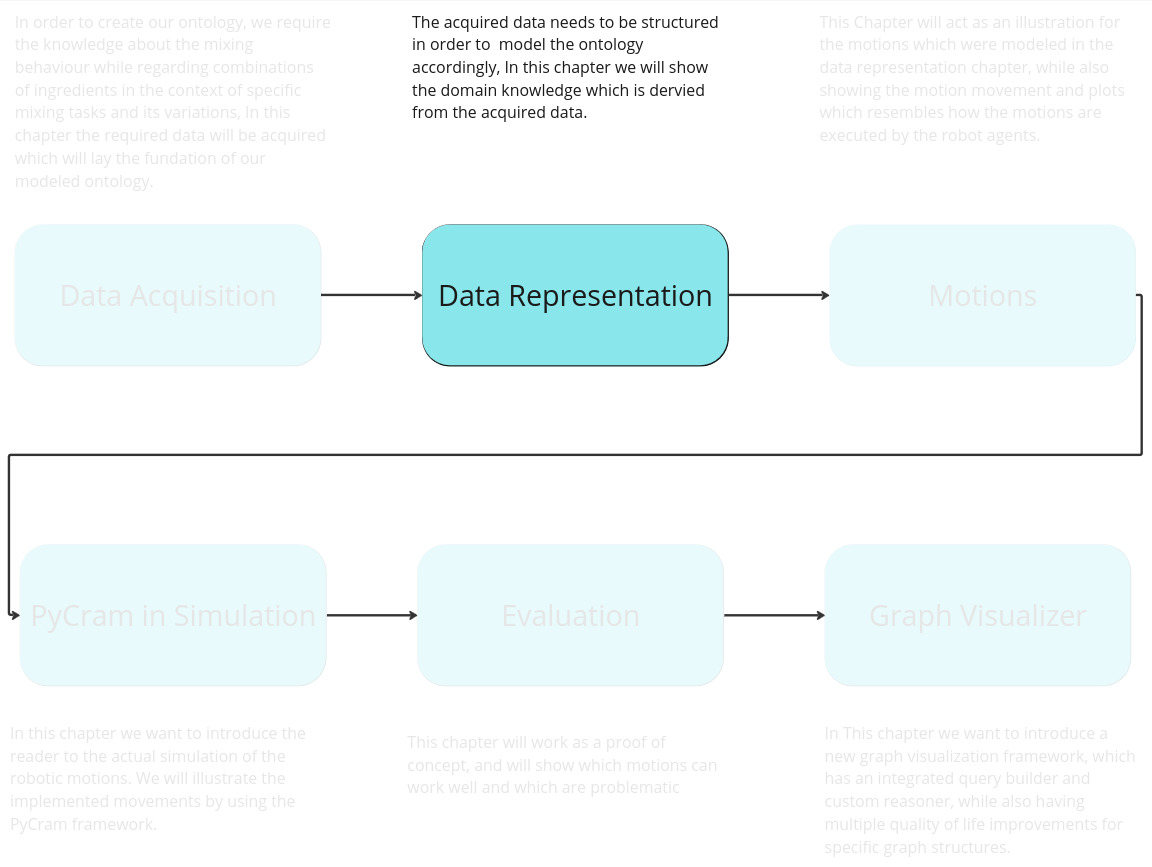
\includegraphics[scale=0.3]{Graphics/overview_2.jpg}
\end{figure}
In this chapter we are going to introduce our modeled knowledge graph which serves as our \textit{OWL} databasis. We modeled several aspects from the acquired data to cover up the full \textit{Mixing} domain. In other words we definde domain knowledge.

Our main goal is to determine different mixing motions from asserted knowledge, like the given task, the set of ingredients used for mixing and additional knowledge like, which container and which tools are used.
Our knowledge base is not overly abstract but not overly simplified either, the robot doesn't learn how to execute motions, but rather it infers motions and its parameters with asserted knowledge, where the inference rules are kept simple.
By simplyfing the knowledgebase, the robot relies on less asserted knowledge, which can result in a higher success rate.

\section{The Knowledgebase}
We designed a Ontology in which we illustrated our needed classes. 
The Knowledgebase is divided upon the superclasses \textit{Ingredient, DesignedTool, Tasks and Motions }
\begin{figure}[H]
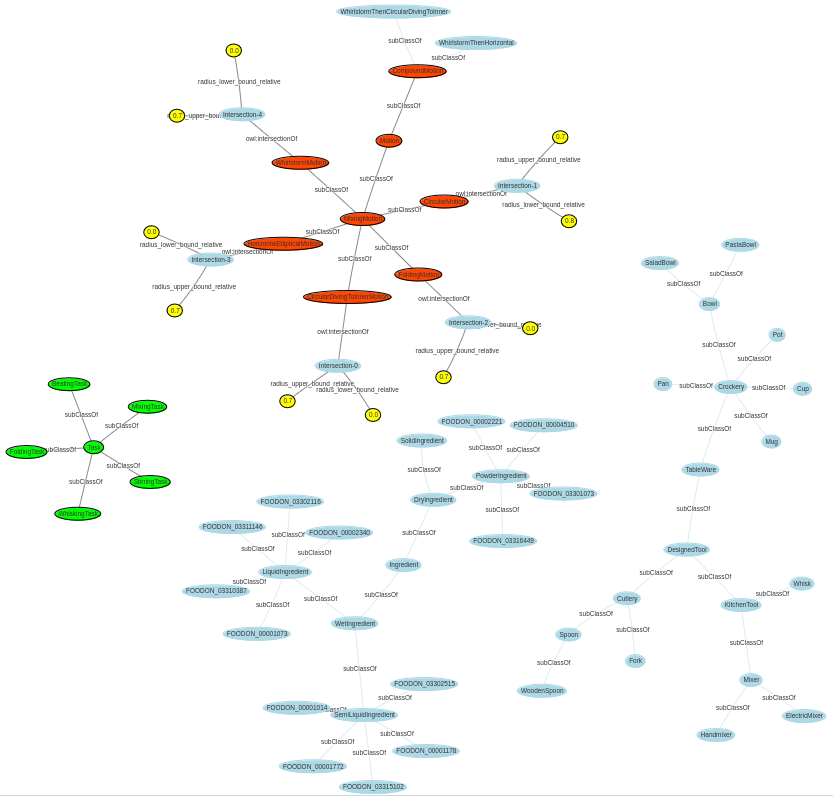
\includegraphics[scale=0.5]{Graphics/mixing_graph_repr.png}
\caption{modeled Knowledgebase}
\end{figure}

\subsection{Ingredients (outdated)}

\textbf{Definition:}
Ingredients are primarily divided into \textit{Dry} and \textit{Wet}, with a need for finer differentiation. More abstracted categories called \textit{Liquid} and \textit{Semi-Liquid} are introduced to encompass finer states such as milk, egg, butter and water. Also additional categories, \textit{Solid} and \textit{Powder}, distinguishes itself from each other by including solid components like vegetables and meat. These distinctions allow for a precise definition of ingredients, enhancing the analysis of mixing motions in the context of cooking/baking and their representation.

\begin{itemize}
    \item \textit{Liquid: Milk, Oil, Water, Vinegar, Vanilla Extract, Sauces}.
    \item \textit{Semi-Liquid: Egg White, Egg yolk, Butter, Whipped Cream}.
    \item \textit{Powder: Flour, Salt, Sugar, Baking Soda, Cocoa Powder}.
    \item \textit{Solid: Onions, Pork, Chicken, Minced meat, Bacon}.
  \end{itemize}

These subsets are also considered the subclasses for the \textbf{Ingredient} superclass.

By importing the concepts from \textit{FoodOn} (CITE HERE), we not only incorporate the specific ingredient we aim to add to the knowledgebase but also automatically acquire all subclasses of those \textit{FoodOn} concepts, once the ontology is imported into ours. 

This approach applies similarly to \nameref{sec:toolsandcontainers} by leveraging \textit{SOMA}, and it can be extended to ingredients through integration with \textit{FoodOn}.


\subsection{Tools and containers}
\label{sec:toolsandcontainers}

By identifying common occuring containers and tools, 
a generalization can be made and this is where \textit{SOMA} helps. \textit{SOMA-Home} is a taxonomy modelling concepts for a kitchen environment.
Top level concepts from \textit{SOMA-Home} can help us identify specific tools and containers without going through dozens of videos. 
Another advantage is, when \textit{SOMA-Home} is extended with new concepts, those concepts can be easily included into the mixing task procedure. 

The tools can be also divided in multiple categories. \textit{Cutlery} consists of \textit{Fork} and \textit{Spoon}, while \textit{Spoon} also has subclasses like a \textit{Wooden Spoon and Tea Spoon}.
Then we have kitchen tools where we can find different types of \textit{mixers} and \textit{whisks}. Last we got the superclass \textit{Crockery} in which our containers we will be saved, like different \textit{Bowls, Pot and Mugs}.

\subsection{Tasks}
Different tasks will be saved under the \textit{Task} superclass. The tasks consists of \textit{Mixing}, which can be regarded as the umbrela term of all tasks, \textit{Stirring} which is mostly a task that includes a circular motion, \textit{Beating} will be mostly used in context with eggs and other wet ingredients, \textit{Folding} which represents a gentle type of mixing and the last task is \textit{Whisking} which is similar to the beating task.
While some of these tasks have only one motion that can be dervied, like the \textit{Folding} task, we discovered that the others tasks can have multiple motions associated to them. This decision is influenced by the set of ingredients on which the motion will be performed

\subsection{Motions (kein Feedback notwendig, muss grundartig geändert werden.)}
The motions are necessary for the robotic system to know what has to be done?. The motions are inferred from Rules that regards a task component, combined with ingredients.
The motion also contain parameters, which should determine the moving space available for the robotic system. As in the mixing world, most of the container have a circular formed base, our motions are defined with a radius.
The most important parameters are:
\begin{itemize}
    \item Radius Lower Bound: This parameter describes the smallest possible radius for a motion. For example if the used container is a bowl, that has a radius of 10 cm, a radius lower bound of 0.1 would imply that the smallest possible radius on which the robot can perform its motion is 1 cm.
    \item Radius Upper Bound: Similar to the radius lower bound, the upper bound determines the maximum radius on which the robot can execute motions.
\end{itemize}
Our implemented motions are:
\begin{itemize}
    \item Circular Motion: A circular motion is a motion defined on a circular with a constant radius. This motion has an equal lower und upper bound radius to keep the radius of the motion constant.  \newline HIER BILD
    \item Whirlstorm Motion: The Whirlstorm motion covers multiple parts of the container, the motion starts on the center of the container and increments its radius until it reaches the radius upper bound parameter, before turning back to the center. \newline HIER BILD
    \item Folding Motion: Folding is a special motion which is mostly used in the context of the folding task. The motion's goal is to mix the ingredients gently without overmixing the mixture. The motion starts on a point on the circle with the radius of the upper bound parameter, from there the motion draws a straight line to the middle point of the container, then getting back to the start point, next the tool will be moved 90 degrees on the defined circle and it moves back to the middle, this motion is repeteadet 4 times, and then you move the tool 20 degrees to cover all of the ingredients before starting the cycle again. \newline HIER BILD
    \item Vertical Circular Motion: The last motion can also be seen as the most difficult one. The main idea of this motion is to `wildly` mix the ingredients. Beschreibung fehlt, Bild hier rein.
\end{itemize}

\section{Rules}
In order to infer the right motion based on the ingredients and task input, rules have to be defined. This rules are \nameref{sec:SWRL}-rules.
In this section we want to illustrate the inference on a high level.
The rules can be thoguht as if conditions, which will then result in a motion, 
for example, if we regard the combination of the task \textit{Mixing} and the ingredient type \textit{Liquid}, we infer the motion \textit{Whirlstormmotion}. 
This can be done for every task and ingredient combination. 
The inference can be illustrated with decision trees which will be shown in the following section for every task and ingredient type combination available. 

\subsection{Mixing}
\begin{figure}[H]
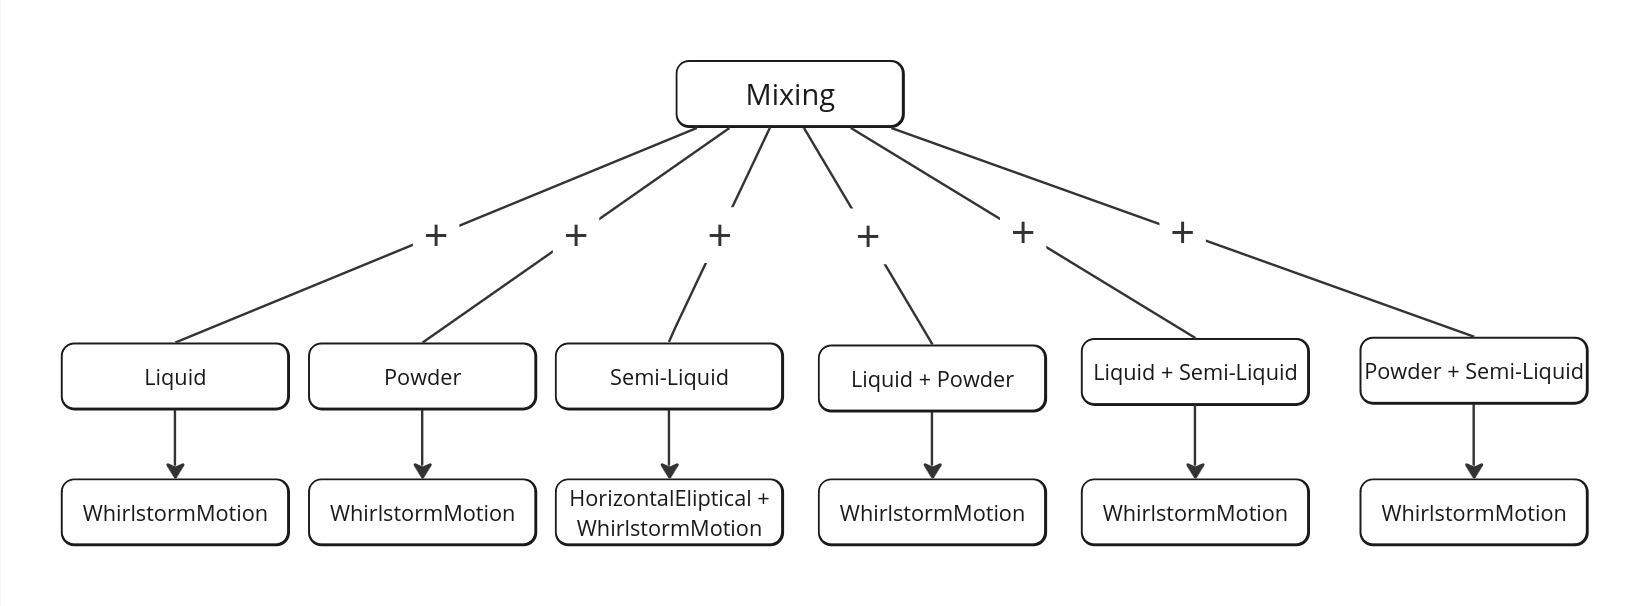
\includegraphics[scale=0.18]{Graphics/MixingDecisionTree.jpg}
\caption{Mixing decision tree}
\end{figure}
\textbf{Definition:} In the context of baking or cooking, a mixing task refers to the process of combining multiple ingredients thoroughly to create a homogeneous mixture. The goal is to distribute the ingredients evenly, ensuring that each component contributes to the overall texture, flavor, and consistency of the final dish or baked good. Mixing is a fundamental step in many recipes and is essential for achieving a balanced and cohesive result (Quelle).


As can be seen from the illustration, the mixing task can primarily be mapped to the Whirlstorm motion. This is not surprising when considering the definition, as this motion results in the uniform distribution of all ingredients in the container.
\subsection{Stirring}
\begin{figure}[H]
    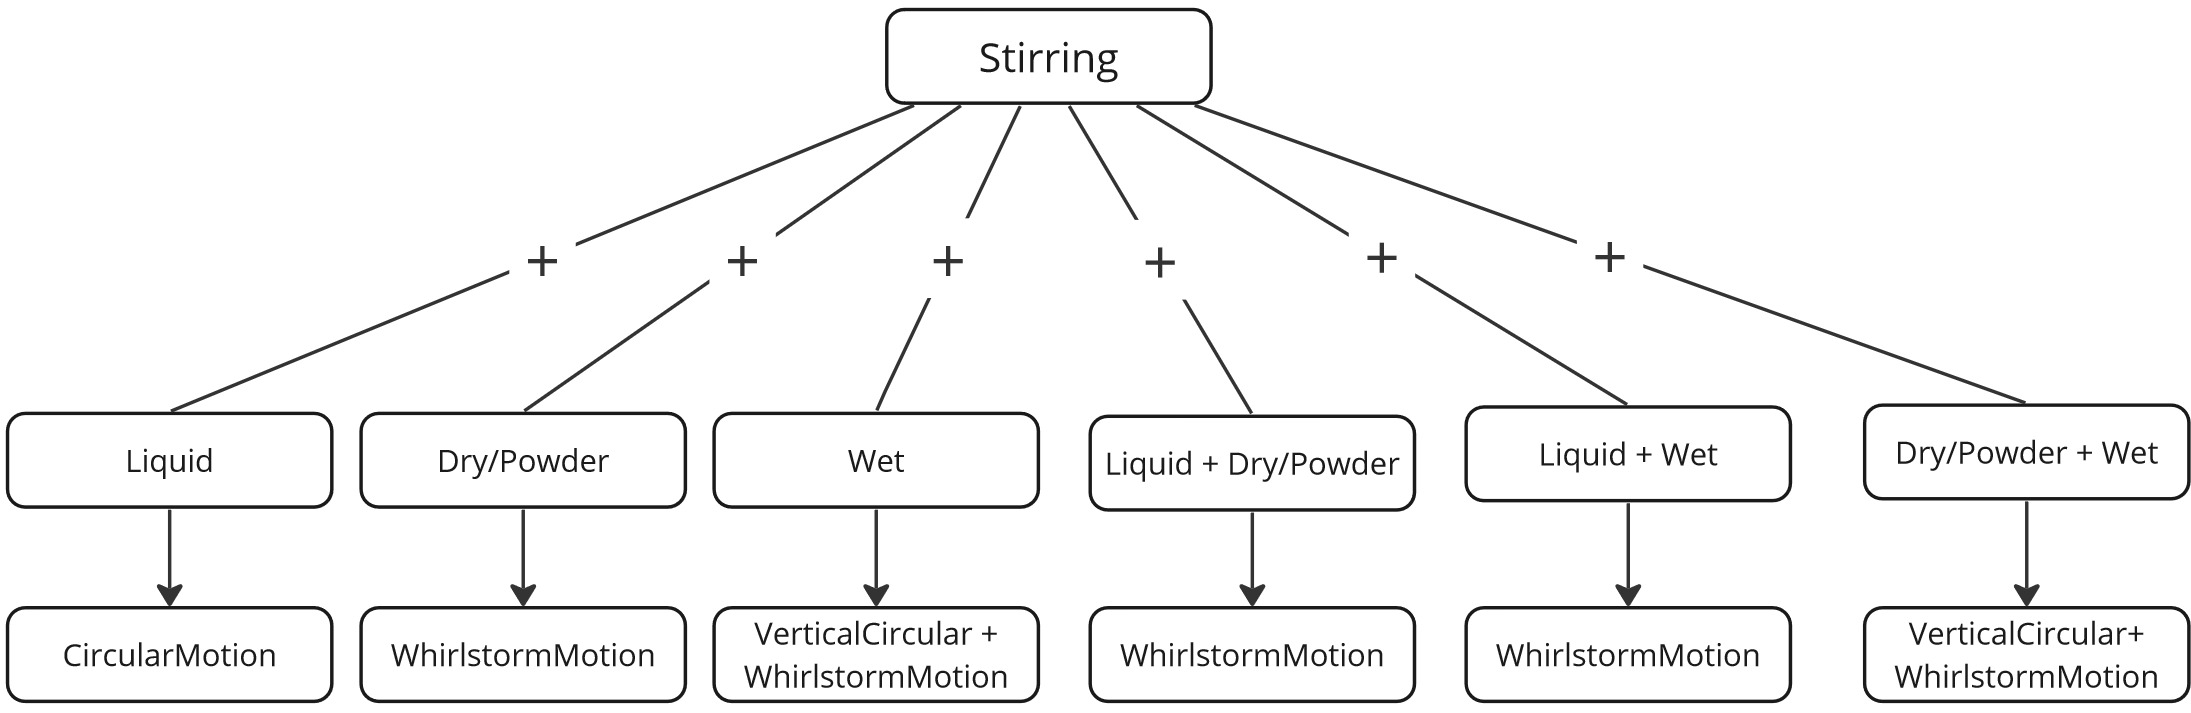
\includegraphics[scale=0.18]{Graphics/StirringDeisionTree.jpg}
    \end{figure}
\textbf{Definition:}
In the context of baking or cooking, a stirring task involves using a utensil, such as a spoon, spatula, or whisk, to agitate and circulate the ingredients within a mixture. The purpose of stirring is to achieve a uniform distribution of ingredients

In comparison to \textit{Mixing}, the \textit{Stirring} task, depending on the ingredients, maps to a broader range of motions. In addition to the \textit{WhirlstormMotion}, the \textit{Circular Motion} is used here for the first time. This is particularly important when considering the \textit{Stirring} task with the ingredient type \textit{Liquid}, as one does not want the ingredients to be whirled, as would be the case with the \textit{Whirlstorm Motion}, but rather just stirred.
\subsection{Beating}
\begin{figure}[H]
    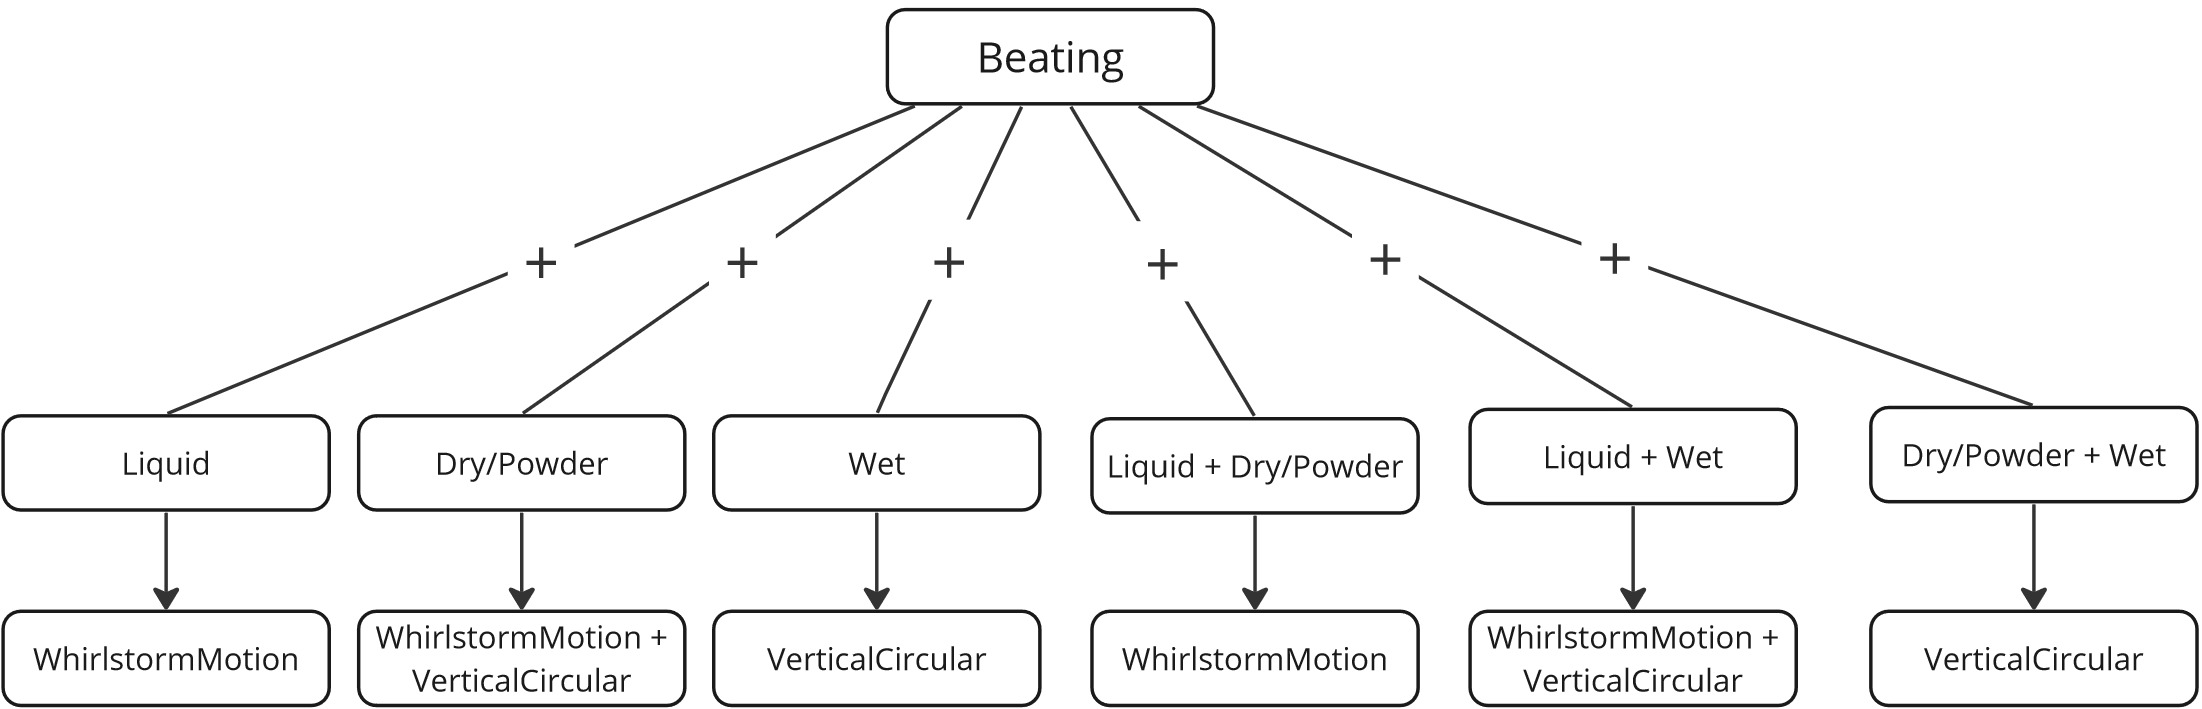
\includegraphics[scale=0.18]{Graphics/BeatingDecisionTree.jpg}
    \end{figure}
\textbf{Definition:}
In the context of baking and cooking, a "beating" task refers to the process of vigorously stirring or mixing ingredients to achieve a specific texture or consistency. Beating is often done to incorporate air into the mixture, create smooth and uniform blends, or alter the physical properties of certain ingredients.

In addition to the Whirlstorm Motion, the Horizontal Eliptic Motion also predominates here. This can be derived from the definition as well, as this motion requires a wild mixing style, to which the Horizontal Eliptic Motion aligns.
\subsection{Whisking}
\begin{figure}[H]
    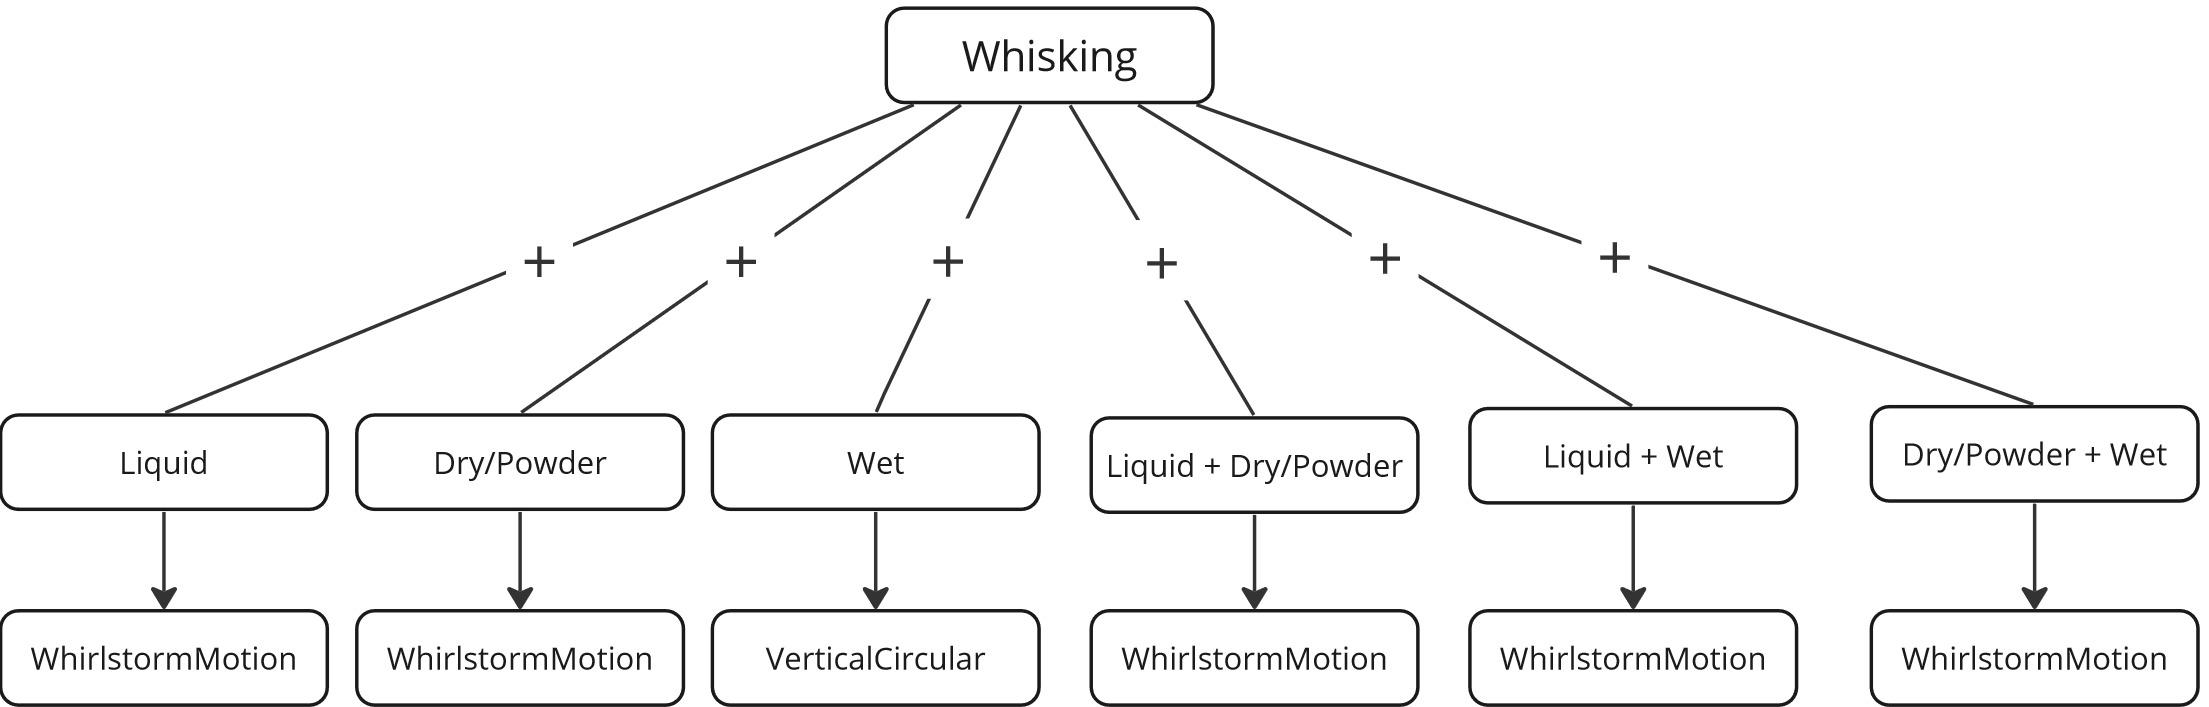
\includegraphics[scale=0.18]{Graphics/WhiskingDecisionTree.jpg}
    \end{figure}
\textbf{Definion:}In the context of baking and cooking, a "whisking" task involves using a kitchen utensil called a whisk to mix, blend, or beat ingredients. A whisk typically consists of wire loops or a coil attached to a handle, and it is designed to incorporate air into mixtures, break up clumps, and create a smooth and uniform texture.

\subsection{Folding}
\begin{figure}[H]
    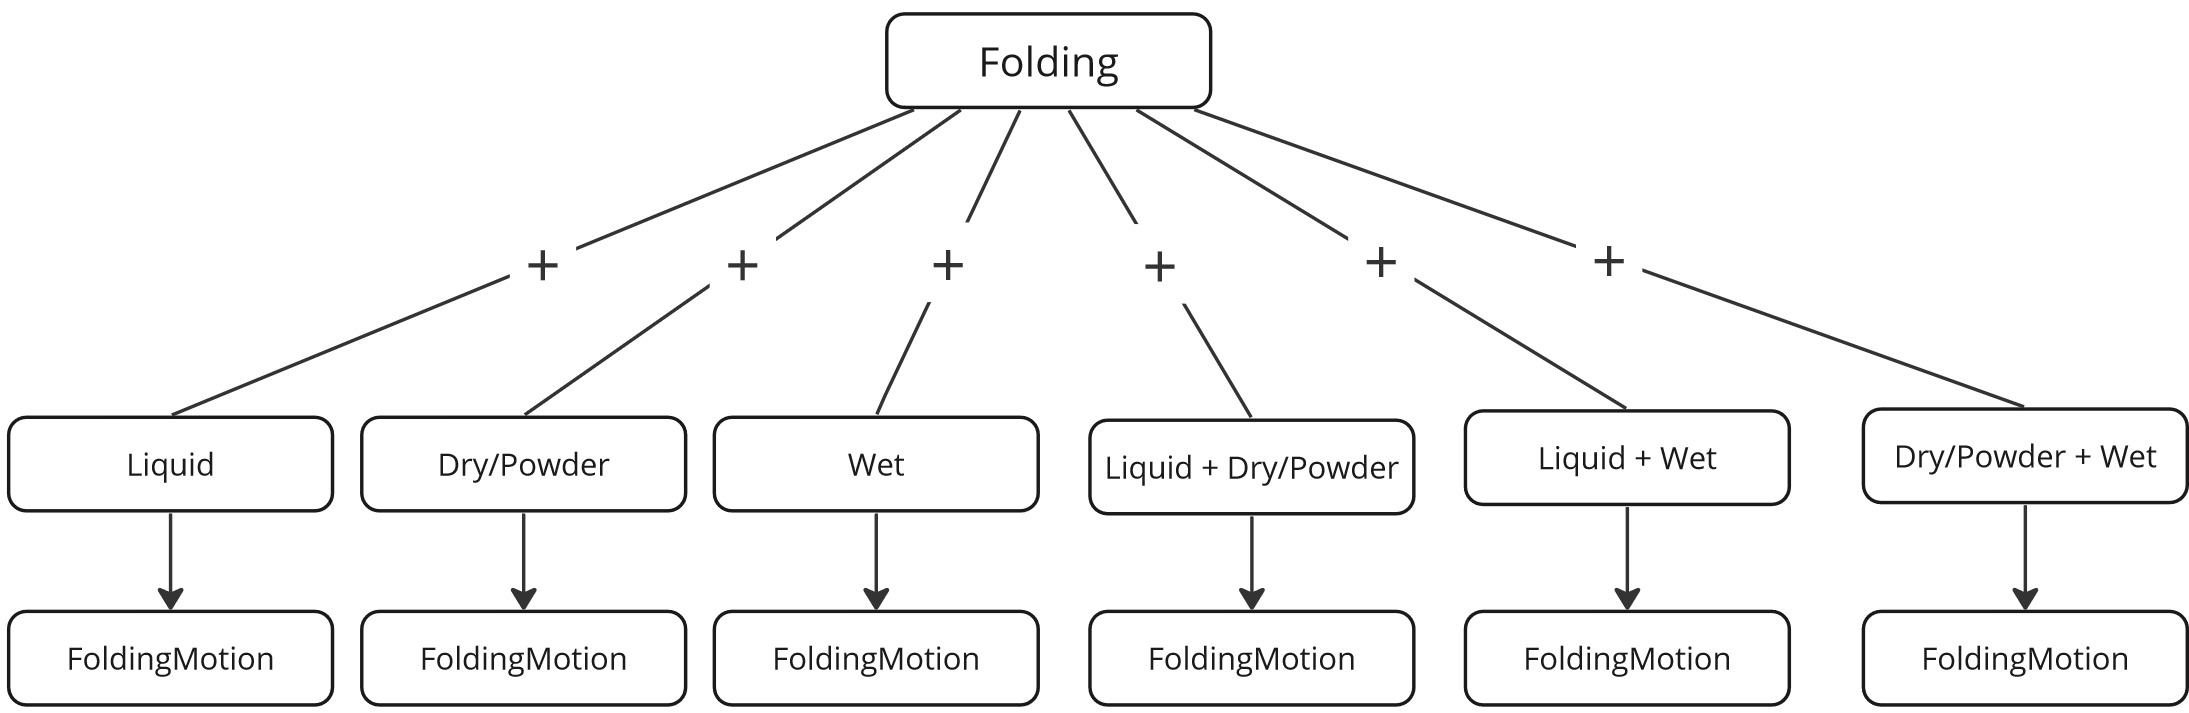
\includegraphics[scale=0.18]{Graphics/FoldingDecisionTree.jpg}
    \end{figure}
\textbf{Definition:}
In the context of baking and cooking, a "folding" task refers to a gentle mixing technique used to incorporate ingredients without deflating or destroying the air bubbles that have been created. Folding is often employed when combining a lighter mixture (such as whipped cream or beaten egg whites) with a denser one (such as a batter or a heavier mixture). The goal is to maintain the desired texture, lightness, or fluffiness in the final dish.

Theoretically, we wouldn't need to graphically represent the Folding Task since each task and ingredient combination maps to a single motion, the Folding Motion. The graphic was nevertheless included for completeness. The Folding Task requires a specific movement that does not remove the air in the mixture, and any other movement would fail.
